\documentclass{sciposter}
\usepackage[brazil]{babel}
\RequirePackage[utf8,utf8x]{inputenc}
\usepackage{url}
\usepackage{multicol}
\usepackage{graphicx}
\usepackage{color}
\usepackage[dvips,dvipdfm,top=0cm,bottom=8cm,left=0cm,right=5cm,paperwidth=80cm,paperheight=100cm]{geometry}

% usar para termos estrangeiros
\newcommand{\eng}[1]{\textit{#1}}
\newcommand{\goiaba}[1]{\textit{Goiaba}}
\newcommand{\code}[1]{\texttt{#1}}

\renewcommand{\fontpointsize}{25pt}

\definecolor{SectionCol}{rgb}{1,1,1}
\definecolor{BoxCol}{rgb}{.230,.230,.76}

\def\abovestrut#1{\rule[0in]{0in}{#1}\ignorespaces}
\def\belowstrut#1{\rule[-#1]{0in}{#1}\ignorespaces}

\def\abovespace{\abovestrut{0.20in}}
\def\aroundspace{\abovestrut{0.20in}\belowstrut{0.10in}}
\def\belowspace{\belowstrut{0.10in}}


\title{\goiaba{}: Um software para processar contornos}
\author{\textbf{Marcos Sampaio e Pedro Kröger}}
\institute{Genos---Grupo de pesquisa em computação musical}
\email{\{mdsmus,pedro.kroger\}@gmail.com}

%% inserir nome do orientador
%% inserir área, sub-área e sub-sub-área

% The following commands can be used to alter the default logo settings
\leftlogo[.7]{ufba-logo}{  % defines logo to left of title (with scale factor)
\rightlogo[1.1]{capes-logo}  % same but on right

\begin{document}

\bibliographystyle{plain}

\conference{\Large \textbf{IX Seminário de Pesquisa e Pós-Graduação---2008
    \hfill \textsf{Grupo de Pesquisa: GENOS}}}

\maketitle

\begin{multicols}{3}

\section{Introdução}

Contornos podem ser entendidos como perfis ou formatos de objetos. Em
Música contornos podem mapear um parâmetro em função de outro, como
altura em função do tempo ou densidade em função da amplitude. São
estruturas manipuláveis através de operações como inversão e
retrogradação. Contornos são importantes porque ajudam a dar coerência
musical a uma obra, assim como conjuntos de notas e motivos.

As figuras \ref{fig:pitches-in-time},
\ref{fig:chord-densities-in-time} e \ref{fig:dynamics-in-time} mostram
o mapeamento de altura, densidade e dinâmica a partir de um contorno
representado graficamente na figura \ref{fig:repr-1023}.

Teorias de contornos
\cite{friedmann85:methodology,morris87:composition,morris93:directions,marvin.ea87:relating,clifford95:contour,polansky.ea92:possible,quinn97:fuzzy,beard03:contour}
têm sido utilizadas em áreas como Percepção e Análise Musical, no
entanto, apesar do atual estado de arte de ferramentas computacionais
aplicadas a música, não existe um sistema computacional para
processamento de contornos que auxilie o compositor ou analista com
tarefas como cálculo automático de operações, plotagem de contornos, e
conversão de partitura para contornos e vice-versa. Por esse motivo
iniciamos o desenvolvimento do \goiaba{}.

Consideramos que contorno é \textbf{um conjunto ordenado de elementos
  distintos, com ou sem repetição, numerados de forma ascendente}
\cite[p. 206]{morris93:directions}. Esta numeração é feita atribuindo
0 para o elemento de menor valor, 1 para o segundo elemento de menor
valor, 2 para o terceiro elemento de menor valor, e assim por
diante. O valor do elemento depende do parâmetro que ele mapeia. Por
exemplo, em um contorno de alturas a nota mais grave tem o menor
valor.

\section{O software Goiaba}

O \goiaba{} é um software desenvolvido na linguagem Common Lisp
\cite{graham94:lisp} e compilado com o SBCL \cite{team07:sbcl}.

Contornos são representados simbolicamente de duas maneiras: como
contornos simples, considerando apenas os valores dos elementos de
contorno \code{(5 9 6)}, e como contornos com duração, considerando
também o local no tempo onde ocorre cada elemento do contorno:
\code{((0 5)(1 9)(2 6))}.

As operações em contornos são implementadas em métodos, aproveitando
do despacho múltiplo usado pelo sistema de objetos de Common Lisp
(CLOS). Desse modo um método como \texttt{transpor} se comporta de
maneira diferente dependendo qual o tipo do seu primeiro parâmetro. No
código da figura \ref{fig:metodos} há dois métodos, sendo o primeiro
para a classe \code{contorno-duracao}, e o segundo para a classe
\code{contorno-simples}.

O \goiaba{} tem diversas operações para lidar com contornos, como
tranposição, inversão, retrogradação, rotação e expansão de
intervalos, como redução de contornos \cite{adams76:melodic}, classe
de contornos equivalentes , série de contornos adjacentes, vetor de
séries de contornos adjacentes, intervalo de contorno, vetor de
intervalo de contorno, vetor de classe de contorno I e II
\cite{friedmann85:methodology} e matriz de comparação
\cite{morris93:directions}.

Finalmente, o \goiaba{} usa a biblioteca Cl-pdf para plotar contornos
definidos, Por exemplo, o código da figura \ref{fig:gera-operacoes}
gera um gráfico com o contorno original, sua transposição,
retrogradação, inversão, rotação, ampliação de altura e inserção de
ponto (figura \ref{fig:operacoes}).

\end{multicols}

\begin{center}

\begin{multicols}{2}

  \begin{figure}
    \centering
    \includegraphics[scale=2]{pitches-in-time}
    \caption{Alturas no tempo}
    \label{fig:pitches-in-time}
  \end{figure}

  \begin{figure}
    \centering
    \includegraphics[scale=2]{chord-densities-in-time}
    \caption{Densidade de acordes no tempo}
    \label{fig:chord-densities-in-time}
  \end{figure}

  \begin{figure}
    \centering
    \includegraphics[scale=2]{dynamics-in-time}
    \caption{Dinâmicas no tempo}
    \label{fig:dynamics-in-time}
  \end{figure}

  \begin{figure}
    \centering
    \includegraphics[scale=2]{c-1023}
    \caption{Representação do contorno (1 0 2 3)}
    \label{fig:repr-1023}
  \end{figure}

\begin{figure}
  \centering
\begin{verbatim}
(defmethod transpor ((objeto contorno-duracao) fator)
  (map-contorno-duracao #L(transpor !1 fator) (pontos objeto)))

(defmethod transpor ((objeto contorno-simples) fator)
  (map-contorno-simples #L(+ !1 fator) (pontos objeto)))
\end{verbatim}
  \label{fig:metodos}
  \caption{Métodos para transposição}
\end{figure}

\begin{figure}
  \centering
\begin{verbatim}
(let ((c1 #d(#p(0 0) #p(1 5) #p(2 3) #p(3 4) #p(4 1) #p(5 3))))
  (plot-page "contornos.pdf"
    (plot-contorno-full 50 500
       c1 "original" :red
       (transpor c1 2) "transposição" :green
       (retrogradar c1) "retrógrado" :blue
       (inverter c1) "inversão" :pink
       (aumentar-altura c1 2) "aumentar-altura" :lightblue
       (rotacionar c1 1) "rotação" :darkcyan
       (insere-ponto c1 '(1 3) 2) "insere ponto" :purple)))
\end{verbatim}
  \label{fig:gera-operacoes}
  \caption{Código para gerar operações}
\end{figure}

\begin{figure}
  \centering
  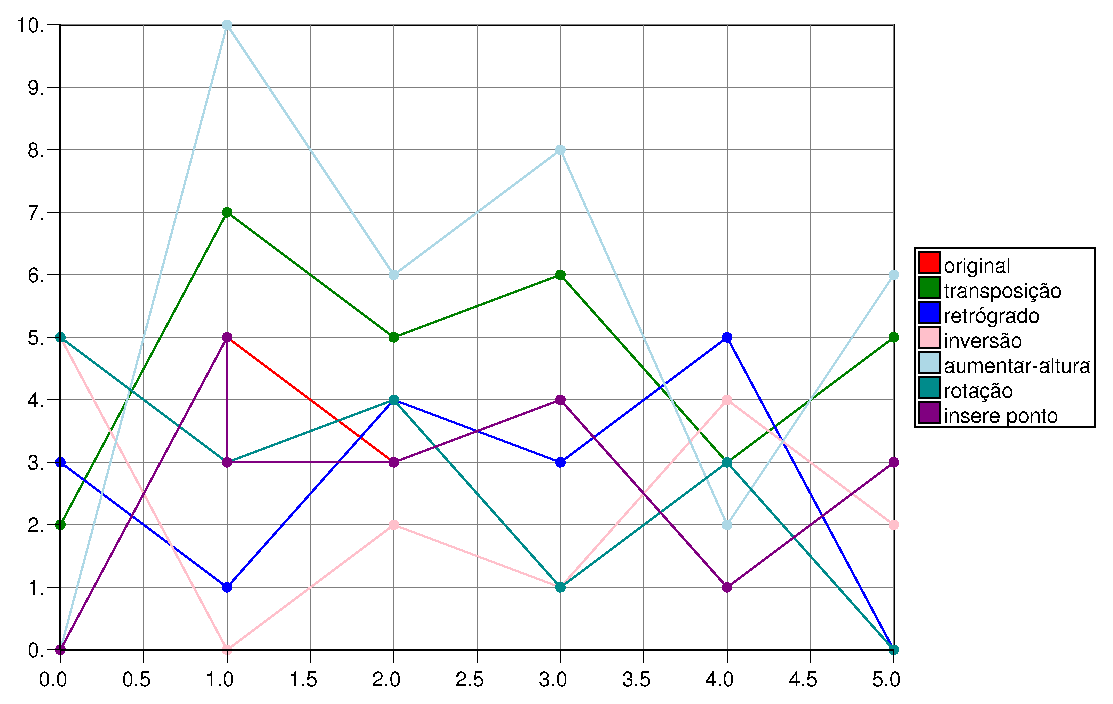
\includegraphics[scale=.9]{contornos}
  \caption{Operações em contorno (0 5 3 4 1 3)}
  \label{fig:operacoes}
\end{figure}

\end{multicols}

\end{center}

\begin{multicols}{3}

\section{Conclusão}

Contornos têm se mostrado úteis para a composição. Até o momento
verificamos a utilidade das operações de inversão, transposição,
retrogradação, rotação, expansão de intervalos, INT$_1$, redução e
preenchimento.

O \goiaba{} tem se mostrado útil tanto para entender contornos quanto
como ferramenta auxiliar à composição musical. Damos prosseguimento ao
seu desenvolvimento com a revisão das teorias de contornos, a
implementação das operações, e a composição de pequenas peças musicais
como experimentos. Esperamos criar uma interface gráfica e via linha
de comando para lançar a primeira versão do software.

\renewcommand{\refname}{Bibliografia}

\bibliography{melodic-contour,music-perception,composition,music-harmony-and-theory,programs,music-analysis,audio,genos,computer-science}

\end{multicols}

\end{document}